
%(BEGIN_QUESTION)
% Copyright 2006, Tony R. Kuphaldt, released under the Creative Commons Attribution License (v 1.0)
% This means you may do almost anything with this work of mine, so long as you give me proper credit

Write an equation for each circuit shown, showing how all the voltages in each circuit relate to each other:

$$\includegraphics[width=15.5cm]{i00387x01.eps}$$

\vskip 10pt

$$\includegraphics[width=15.5cm]{i00387x02.eps}$$

\vfil \eject

$$\includegraphics[width=15.5cm]{i00387x03.eps}$$

\vskip 10pt

$$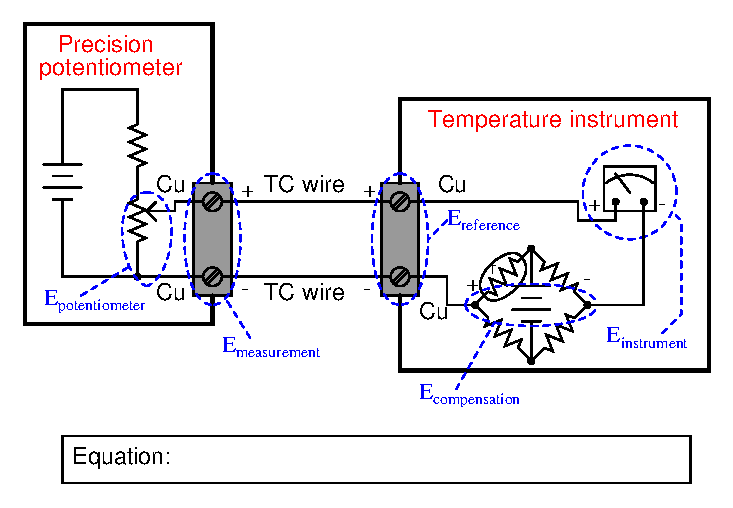
\includegraphics[width=15.5cm]{i00387x04.eps}$$

\vskip 20pt \vbox{\hrule \hbox{\strut \vrule{} {\bf Suggestions for Socratic discussion} \vrule} \hrule}

\begin{itemize}
\item{} You should notice a definite progression in complexity from the first circuit to the last in this question.  Why do you suppose these circuits were arranged in this order?  How might this help you figure out the equation for a realistic calibration circuit (such as the last two) in the future if you do not have a reference at hand to remind you how thermocouple circuits work?
\end{itemize}

\underbar{file i00387}
%(END_QUESTION)





%(BEGIN_ANSWER)

$$\includegraphics[width=15.5cm]{i00387x05.eps}$$

\vskip 10pt

$$\includegraphics[width=15.5cm]{i00387x06.eps}$$

\vskip 10pt

$$\includegraphics[width=15.5cm]{i00387x07.eps}$$

\vskip 10pt

$$\includegraphics[width=15.5cm]{i00387x08.eps}$$

\vskip 10pt

To make this really simple: if you desire to know the proper potentiometer setting for generating an indication on any thermocouple-based instrument, just look up the millivoltage for the desired temperature, and subtract the millivoltage corresponding to the temperature at the point where either (A) copper wires join to a compensated instrument, or (B) where thermocouple wires join to an internally-copper, uncompensated, calibration device (assuming the temperature at the calibration device is the same as the temperature of the measuring instrument).

%(END_ANSWER)





%(BEGIN_NOTES)


%INDEX% Measurement, temperature: thermocouple circuit equations

%(END_NOTES)


